\documentclass[class=report, float=false, crop=false]{standalone}

\usetheme{Warsaw}
% \usecolortheme{spruce}

%%%%% PACKAGES

\usepackage{graphicx} % figures
\usepackage{multimedia} % videos
\usepackage{url}
\usepackage{amsmath}
\usepackage{amssymb}
\everymath{\displaystyle}
\usepackage{epstopdf} % conversion from .eps to .pdf
\usepackage[utf8]{inputenc}
\usepackage[T1]{fontenc}
\usepackage{upgreek}
\usepackage{nameref}
\usepackage{url}
\usepackage{pgf, tikz}
\usepackage{float}
\usepackage[english]{babel}
\usepackage{caption}
\usepackage{subcaption}
\usepackage{fontawesome5}
\usepackage{xcolor}

\usepackage{biblatex}
\addbibresource{references/biblio.bib}

%%%%% TEMPLATE

\captionsetup{font=scriptsize,labelfont={scriptsize, color=blue}}

\AtBeginSubsection[]
{
 \begin{frame}<beamer>{}
   \tableofcontents[currentsection,currentsubsection]
 \end{frame}
}
\AtBeginSection[]
{
  \begin{frame}<beamer>{}
    \tableofcontents[currentsection]
  \end{frame}
}

\defbeamertemplate*{footline}{mytheme}%
{  \begin{beamercolorbox}[ht=2.5ex]{bordure}
\begin{beamercolorbox}[wd=0.2\paperwidth,ht=2.5ex,dp=1ex,center]{author in head/foot}%
\usebeamerfont{author in head}\insertshortauthor
\end{beamercolorbox}%
\begin{beamercolorbox}[wd=0.57\paperwidth,ht=2.5ex,dp=1ex,center]{title in head/foot}%
\usebeamerfont{title in head/foot}\insertshorttitle
\end{beamercolorbox}%
% \begin{beamercolorbox}[wd=0.4\paperwidth,ht=2.5ex,dp=1ex,center]{title in head/foot}%
% \usebeamerfont{title in head/foot}\insertdate
% \end{beamercolorbox}%
\begin{beamercolorbox}[wd=0.12\paperwidth,ht=2.5ex,dp=1ex,center]{title in head/foot}%
\usebeamerfont{title in head/foot}\insertdate
\end{beamercolorbox}%
\begin{beamercolorbox}[wd=0.11\paperwidth,ht=2.5ex,dp=1ex,center]{date in head/foot}%
\usebeamerfont{date in head/foot}\insertframenumber /\inserttotalframenumber{}\hspace{2ex}
\end{beamercolorbox}%

  \end{beamercolorbox}
}

% \defbeamertemplate*{headline}{mytheme}%
% {  \begin{beamercolorbox}[ht=2.5ex]{bordure}
% \begin{beamercolorbox}[wd=\paperwidth,ht=2.5ex,dp=2ex]{author in head/foot}%
% \usebeamerfont{author in head}\vskip6pt\insertsectionnumber.~\insertsection \hfill \insertsubsection
% \end{beamercolorbox}%
%
%   \end{beamercolorbox}
% }

\makeatletter
\let\insertsupervisor\relax
\newcommand\supervisortitle{supervised by}
\mode<all>
{
  \newcommand\supervisor[1]{\def\insertsupervisor{#1}}
  \titlegraphic{}
}
\defbeamertemplate*{title page}{supdefault}[1][]
{
  \vbox{}
  \vfill
  \begingroup
    \centering
    \begin{beamercolorbox}[sep=8pt,center,#1]{title}
      \usebeamerfont{title}\inserttitle\par%
      \ifx\insertsubtitle\@empty\relax%
      \else%
        \vskip0.25em%
        {\usebeamerfont{subtitle}\usebeamercolor[fg]{subtitle}\insertsubtitle\par}%
      \fi%
    \end{beamercolorbox}%
    \vskip1em\par
    \begin{beamercolorbox}[sep=8pt,center,#1]{author}
      \usebeamerfont{author}\textbf{\insertauthor}
    \end{beamercolorbox}
    \vspace{-10pt}
    \ifx\insertsupervisor\relax\relax\else
    \begin{beamercolorbox}[sep=8pt,center,#1]{author}
      \usebeamerfont{author}{\footnotesize \supervisortitle}~{\small\insertsupervisor}
    \end{beamercolorbox}\fi
    \vspace{-5pt}
    \begin{beamercolorbox}[sep=8pt,center,#1]{date}
      \usebeamerfont{date}\insertdate
    \end{beamercolorbox}\vskip0.5em
    {\usebeamercolor[fg]{titlegraphic}\inserttitlegraphic\par}
  \endgroup
  \vfill
}
\setbeamertemplate{title page}[supdefault][colsep=-4bp,rounded=true,shadow=\beamer@themerounded@shadow]\makeatother

\setbeamerfont{footnote}{size=\tiny}

\makeatletter
\newlength\beamerleftmargin
\setlength\beamerleftmargin{\Gm@lmargin}
\makeatother

%%%%% COMMANDS

\providecommand\blfootnote[1]{%
  \begingroup
  \renewcommand\thefootnote{}\footnote{#1}%
  \addtocounter{footnote}{-1}%
  \endgroup
}

\providecommand\encircle[1]{%
  \tikz[baseline=(X.base)]
    \node (X) [draw, shape=circle, inner sep=0] {\strut #1};}

\providecommand{\appropto}{\mathrel{\vcenter{
  \offinterlineskip\halign{\hfil$##$\cr
    \propto\cr\noalign{\kern2pt}\sim\cr\noalign{\kern-2pt}}}}}

\setbeamertemplate{blocks}[rounded][shadow=true]

\providecommand{\isEquivTo}[1]{\underset{#1}{\sim}}

\providecommand{\appropto}{\mathrel{\vcenter{
  \offinterlineskip\halign{\hfil$##$\cr
    \propto\cr\noalign{\kern2pt}\sim\cr\noalign{\kern-2pt}}}}}

\makeatletter
\providecommand{\subalign}[1]{%
  \vcenter{%
    \Let@ \restore@math@cr \default@tag
    \baselineskip\fontdimen10 \scriptfont\tw@
    \advance\baselineskip\fontdimen12 \scriptfont\tw@
    \lineskip\thr@@\fontdimen8 \scriptfont\thr@@
    \lineskiplimit\lineskip
    \ialign{\hfil$\m@th\displaystyle##$&$\m@th\displaystyle{}##$\crcr
      #1\crcr
    }%
  }
}
\makeatother


\graphicspath{{figures/images/}{figures/figs/}}

\begin{document}

\chapter{Shear strain correlation}
\label{chap:strain}

\section{Plastic deformation}
\label{section:plastic_deformation}

% explain the origin of plastic flow, the build up of shear strain correlations, their characteristics

Current theories of plastic deformation of amorphous solids rely on the existence of \textit{shear transformation zones}, which are special sites, a few particles wide, where particles are able to rearrange themselves in response to applied stresses \cite{falk1998dynamics}. Plastic deformation is then the consequence of localized irreversible rearrangements, coupled by elastic strain fields \cite{nicolas2014spatiotemporal} which are solutions of the Eshelby inclusion problem \cite{eshelby1959elastic}.\\

These plastic rearrangements, coupled in an elastic medium, have also been observed in supercooled liquids near the glass transition \cite{chattoraj2013elastic, illing2016strain, hassani2018long}, hence the claim that supercooled liquids are "solids that flow" \cite{dyre2006colloquium}.\\

With $\varepsilon_{xy}(\vec{r}, t, t + \Delta t)$ the accumulated shear strain at position $\vec{r}$ and between times $t$ and $t + \Delta t$ (see section \ref{subsection:shear_strain}), we have in these systems that $C_{\varepsilon_{xy}\varepsilon_{xy}}(\Delta \vec{r}, \Delta t)$, its autocorrelation function (see section \ref{subsection:shear_strain_correlation}), has the same quadrupolar symmetry and algebraic decay far from the origin as the strain field \cite{illing2016strain, hassani2018long}, \textit{i.e.}
\begin{equation}
C_{\varepsilon_{xy}\varepsilon_{xy}}(\Delta \vec{r}, \Delta t) \underset{\frac{||\Delta \vec{r}||}{a} \gg 1}{\propto} \frac{\cos4\theta}{||\Delta \vec{r}||^2}
\label{css_eshelby}
\end{equation}
in 2 dimensions, with $a$ the average interparticle distance.\\

In this chapter, we aim at determining if the transition from the fluid to the phase separated regime is associated with the development of algebraic shear strain correlations.

\section{Shear strain}

\subsection{Shear strain}
\label{subsection:shear_strain}

With $\vec{u}(\vec{r}, t, t + \Delta t) = \begin{pmatrix} u_x(\vec{r}, t, t + \Delta t) \\ u_y(\vec{r}, t, t + \Delta t) \end{pmatrix}$ the displacement of particle at position $\vec{r}$ at time $t$ between times $t$ and $t + \Delta t$, we introduce the linearised strain tensor $\rttensor{\varepsilon}$ \cite{landau1986theory}
\begin{equation}
\begin{aligned}
&\rttensor{\varepsilon}(\vec{r}, t, t + \Delta t)\\
\underset{\frac{||\vec{u}||}{L} \ll 1}{=} &\begin{pmatrix} \frac{\partial}{\partial x} u_x(\vec{r}, t, t + \Delta t) & \frac{1}{2} \left(\frac{\partial}{\partial y} u_x(\vec{r}, t, t + \Delta t) + \frac{\partial}{\partial x} u_y(\vec{r}, t, t + \Delta t)\right) \\ \frac{1}{2} \left(\frac{\partial}{\partial y} u_x(\vec{r}, t, t + \Delta t) + \frac{\partial}{\partial x} u_y(\vec{r}, t, t + \Delta t)\right) &  \frac{\partial}{\partial y} u_y(\vec{r}, t, t + \Delta t) \end{pmatrix}
\end{aligned}
\end{equation}
with $L$ the characteristic length of the system, in which we will consider only the diagonal terms, $\textit{i.e.}$ the linearised shear strain
\begin{equation}
\varepsilon_{xy}(\vec{r}, t, t + \Delta t) = \varepsilon_{yx} = \frac{1}{2} \left(\frac{\partial}{\partial y} u_x(\vec{r}, t, t + \Delta t) + \frac{\partial}{\partial x} u_y(\vec{r}, t, t + \Delta t)\right)
\label{linearised_shear_strain}
\end{equation}
which characterises the deformation of the system perpendicularly to the direction of deformation.

\subsection{Shear strain correlation}
\label{subsection:shear_strain_correlation}

We define the shear strain correlation, which is the auto-correlation function of the linearised shear strain introduced in equation \ref{linearised_shear_strain}
\begin{equation}
\begin{aligned}
C_{\varepsilon_{xy}\varepsilon_{xy}}(\Delta \vec{r}, \Delta t) &= \left<\varepsilon_{xy}(\vec{r}+\Delta\vec{r}, t, t + \Delta t)\varepsilon_{xy}(\vec{r}, t, t + \Delta t)\right>_{\vec{r}, t}\\
&= \frac{\int dt \int d^2\vec{r}~ \varepsilon_{xy}(\vec{r}, t, t+\Delta t)\varepsilon_{xy}(\vec{r} + \Delta \vec{r}, t, t+\Delta t)}{\int dt \int d^2\vec{r}~ |\varepsilon_{xy}(\vec{r}, t, t+\Delta t)|^2}\\
&= \frac{\mathcal{F}^{-1}\{\int dt~ |\mathcal{F}\{\varepsilon_{xy}\}(\vec{k}, t, t + \Delta t)|^2\}(\Delta \vec{r}, \Delta t)}{\int dt \int d^2\vec{r}~ ||\varepsilon_{xy}(\vec{r}, t, t+\Delta t)||^2}
\end{aligned}
\label{Css}
\end{equation}
where we refer to appendix \ref{field_auto_correlation} for calculation details leading to the last line of equation \ref{Css}.\\

As discussed in section \ref{section:plastic_deformation}, we expect $C_{\varepsilon_{xy}\varepsilon_{xy}}(\Delta \vec{r}, \Delta t)$ to have a four-fold symmetry. Inspired by \cite{illing2016strain}, we then introduce the projection of the shear strain correlation on $\cos4\theta$
\begin{equation}
C_4^4(\Delta r, \Delta t) = \frac{1}{\pi} \int_0^{2\pi} d\theta~ \cos(4\theta)~ C_{\varepsilon_{xy}\varepsilon_{xy}}(\Delta\vec{r}\equiv(\Delta r, \theta), \Delta t)
\label{c44_definition}
\end{equation}
which in a 2D elastic medium should decay algebraically far from the origin
\begin{equation}
C_4^4(\Delta r, \Delta t) \underset{\frac{\Delta r}{a} \gg 1}{\propto} \frac{1}{\Delta r^2}
\end{equation}
where $a$ is the average interparticle distance.

\section{Real space method}

\subsection{Method}

\myparagraph{Coarse-graining}

We only have access to discrete particle positions to calculate displacements. In order to obtain smooth strain fields, we then have to go through some sort of coarse-graining of these displacements.\\

On the basis of a method detailed in \cite{goldhirsch2002microscopic}, we define the coarse-graining operator $\mathcal{A}(\sigma, r_c)$ which associates to any particle-dependent variable $c_i(t)$ its coarse-grained version $\bar{c}(\vec{r}, t)$ such that
\begin{equation}
\bar{c}(\vec{r}, t) = \mathcal{A}(\sigma, r_c)\{c_i(t)\} = \sum_{i=1}^N c_i(t) \phi(\vec{r}-\vec{r}_i(t), \sigma, r_c)
\end{equation}
where $\phi(\vec{r}, \sigma, r_c)$ is a normalised non-negative coarse-graining function, with a single maximum at $\vec{r} = \vec{0}$, of width $\sigma$ -- the coarse-graining scale -- and cut-off radius $r_c$.\\

As has been done in \cite{illing2016strain}, we choose a Gaussian coarse-graining function $\phi(\vec{r}, \sigma, r_c)$ of width $\sigma$ with a cut-off radius $r_c$
\begin{equation}
\phi(\vec{r}, \sigma, r_c) = \frac{1}{\mathcal{N}(\sigma, r_c)} \begin{cases} \exp\left(-\frac{||\vec{r}||^2}{2\sigma^2}\right) &\text{ if } ||\vec{r}|| < r_c \\ 0 & \text{ otherwise} \end{cases}
\end{equation}
where $\mathcal{N}(\sigma, r_c)$ normalises the function, \textit{i.e.} is such that
\begin{equation}
\int_{\mathbb{R}^2} d^2\vec{r}~ \phi(\vec{r}, \sigma, r_c) = \frac{1}{\mathcal{N}(\sigma, r_c)}\int_0^{r_c} dr~ 2 \pi r \exp\left(-\frac{r^2}{2\sigma^2}\right) = 1 \Leftrightarrow \mathcal{N}(\sigma, r_c) = 2\pi\sigma^2\left(1 - \exp\left(-\frac{r_c^2}{2\sigma^2}\right)\right)
\end{equation}
It is straightforward to verify that this coarse-graining function satisfies the aforementioned conditions.\\

We then define the coarse-grained displacement field \cite{illing2016strain}
\begin{equation}
\bar{\vec{u}}(\vec{r}, t, t+\Delta t) = \frac{1}{\bar{\rho}(\vec{r}, t)} \mathcal{A}(\sigma, r_c)\{\vec{u}(\vec{r}_i(t), t, t+\Delta t)\} = \frac{1}{\bar{\rho}(\vec{r}, t)} \sum_{i=1}^N \vec{u}(\vec{r}_i(t), t, t+\Delta t) \phi(\vec{r}-\vec{r}_i(t), \sigma, r_c)
\label{coarse_grained_u}
\end{equation}
where $\bar{\rho}(\vec{r}, t)$ is the coarse-grained density
\begin{equation}
\bar{\rho}(\vec{r}, t) = \mathcal{A}(\sigma, r_c)\{m_i\} = \sum_{i=1}^N m_i \phi(\vec{r}-\vec{r}_i(t), \sigma, r_c)
\end{equation}
with $m_i$ the mass of particle $i$.\\

It follows, from equations \ref{linearised_shear_strain} and \ref{coarse_grained_u}, the expression of the linearised shear strain from the coarse-grained displacements
\begin{equation}
\begin{aligned}
\varepsilon_{xy}(\vec{r}, t, t + \Delta t) &= \frac{1}{2} \left(\frac{\partial}{\partial x}\bar{u}_y(\vec{r}, t, t + \Delta t) + \frac{\partial}{\partial y}\bar{u}_x(\vec{r}, t, t + \Delta t)\right)\\
&= \frac{1}{2}\begin{aligned}[t]\Bigg[&\frac{\partial}{\partial x}\left(\frac{1}{\bar{\rho}(\vec{r}, t)}\right)\underbrace{\sum_{i=1}^N u_y(\vec{r}_i(t), t, t + \Delta t)\phi(\vec{r} - \vec{r}_i(t), \sigma, r_c)}_{\displaystyle\mathcal{A}(\sigma, r_c)\{u_y(\vec{r}_i(t), t, t + \Delta t)\}}\\
&+ \frac{1}{\bar{\rho}(\vec{r}, t)}\sum_{i=1}^N u_y(\vec{r}_i(t), t, t + \Delta t) \frac{\partial}{\partial x}\left(\phi(\vec{r} - \vec{r}_i(t), \sigma, r_c)\right)\\
&+ \frac{\partial}{\partial y}\left(\frac{1}{\bar{\rho}(\vec{r}, t)}\right)\underbrace{\sum_{i=1}^N u_x(\vec{r}_i(t), t, t + \Delta t)\phi(\vec{r} - \vec{r}_i(t), \sigma, r_c)}_{\displaystyle\mathcal{A}(\sigma, r_c)\{u_x(\vec{r}_i(t), t, t + \Delta t)\}}\\
&+ \frac{1}{\bar{\rho}(\vec{r}, t)}\sum_{i=1}^N u_x(\vec{r}_i(t), t, t + \Delta t) \frac{\partial}{\partial x}\left(\phi(\vec{r} - \vec{r}_i(t), \sigma, r_c)\right)\Bigg]\end{aligned}
\end{aligned}
\end{equation}
where we have, $\forall \vec{r}$ such that $||\vec{r}|| < r_c$,
\begin{equation}
\begin{aligned}
\frac{\partial}{\partial \vec{r}}\phi(\vec{r} - \vec{r}_i(t), \sigma, r_c) &= \frac{1}{\mathcal{N}(\sigma, r_c)}\frac{\partial}{\partial\vec{r}} \exp\left(-\frac{||\vec{r} - \vec{r}_i(t)||^2}{2\sigma^2}\right)\\
&= - \frac{\vec{r} - \vec{r}_i(t)}{\mathcal{N}(\sigma, r_c)\sigma^2} \exp\left(-\frac{||\vec{r} - \vec{r}_i(t)||^2}{2\sigma^2}\right)\\
&= - \frac{\vec{r} - \vec{r}_i(t)}{\sigma^2}\phi(\vec{r} - \vec{r}_i(t), \sigma, r_c)
\end{aligned}
\end{equation}
which result can be extrapolated to any $\vec{r}$, and from which it directly follows for any particle-dependent variable $c_i(t)$ that
\begin{equation}
\begin{aligned}
\frac{\partial}{\partial \vec{r}} \bar{c}(\vec{r}, t) &= \sum_{i=1}^N c_i(t) \frac{\partial}{\partial \vec{r}} \phi(\vec{r} - \vec{r}_i(t), \sigma, r_c)\\
&= -\frac{1}{\sigma^2} \sum_{i=1}^N c_i(t) (\vec{r} - \vec{r}_i(t)) \phi(\vec{r} - \vec{r}_i(t), \sigma, r_c)\\
&= -\frac{1}{\sigma^2} \mathcal{A}(\sigma, r_c)\left\{c_i(t)(\vec{r} - \vec{r}_i(t))\right\}
\end{aligned}
\end{equation}
and thus for the coarse-grained density in particular
\begin{equation}
\begin{aligned}
\frac{\partial}{\partial\vec{r}} &= -\frac{1}{\bar{\rho}^2(\vec{r}, t)} \frac{\partial}{\partial\vec{r}} \bar{\rho}(\vec{r}, t)\\
&= \frac{1}{\bar{\rho}^2(\vec{r}, t)\sigma^2} \mathcal{A}(\sigma, r_c)\left\{m_i(\vec{r} - \vec{r}_i(t))\right\}
\end{aligned}
\end{equation}
which finally leads to the expression of the linearised shear strain as function of the positions, masses and displacements of the particles, and the coarse-grained density
\begin{equation}
\begin{aligned}
\varepsilon_{xy}(\vec{r}, t, t + \Delta t) = \frac{1}{2}
&\begin{aligned}[t]\Bigg[\frac{1}{\bar{\rho}^2(\vec{r}, t)\sigma^2} \Big(&\mathcal{A}(\sigma, r_c)\left\{m_i(y - y_i(t))\right\} \times \mathcal{A}(\sigma, r_c)\left\{u_x(\vec{r}_i(t), t, t + \Delta t)\right\} \\ + &\mathcal{A}(\sigma, r_c)\left\{m_i(x - x_i(t))\right\} \times \mathcal{A}(\sigma, r_c)\left\{u_y(\vec{r}_i(t), t, t + \Delta t)\right\}\Big)\end{aligned}\\
& \begin{aligned}[t]-\frac{1}{\bar{\rho}(\vec{r}, t)\sigma^2} \Big(&\mathcal{A}(\sigma, r_c)\left\{u_x(\vec{r}_i(t), t, t + \Delta t)(y - y_i(t))\right\} \\ + &\mathcal{A}(\sigma, r_c)\left\{u_y(\vec{r}_i(t), t, t + \Delta t)(x - x_i(t))\right\}\Big)\Bigg]\end{aligned}
\end{aligned}
\label{linearised_cg_shear_strain}
\end{equation}

\myparagraph{Computation details}

We divide the system square box in $N_{cases} \times N_{cases}$ linearly spaced square boxes with centres $(\vec{R}_{kl})_{1 \leq k,l \leq N_{cases}}$. We then choose $S_{max}$ times $(t_m)_{1 \leq m \leq S_{max}}$, with $\forall m$, $t_m \geq S_{init}$.\\

In our model, we consider $\forall i \in \llbracket 1; N \rrbracket$, $m_i = 1$.\\

We then have $S_{max}$ grids of linearised shear strain $(\varepsilon_{xy,kl}(t_m, t_m + \Delta t))_{1 \leq k, l \leq N_{cases}}$, defined $\forall k,l \in \llbracket 1; N_{cases} \rrbracket$ by
\begin{equation}
\begin{aligned}
\varepsilon_{xy,kl}(t_m, t_m + \Delta t) = \frac{1}{2}
&\begin{aligned}[t]\Bigg[\frac{1}{\bar{\rho}^2(\vec{R}_{kl} ,t_m)\sigma^2} \Big(&\mathcal{A}(\sigma, r_c)\left\{Y_{kl} - y_i(t_m)\right\} \times \mathcal{A}(\sigma, r_c)\left\{u_x(\vec{r}_i(t_m), t_m, t_m + \Delta t)\right\} \\ + &\mathcal{A}(\sigma, r_c)\left\{X_{kl} - x_i(t)\right\} \times \mathcal{A}(\sigma, r_c)\left\{u_y(\vec{r}_i(t_m), t_m, t_m + \Delta t)\right\}\Big)\end{aligned}\\
& \begin{aligned}[t]-\frac{1}{\bar{\rho}(\vec{R}_{kl}, t_m)\sigma^2} \Big(&\mathcal{A}(\sigma, r_c)\left\{u_x(\vec{r}_i(t), t_m, t_m + \Delta t)(Y_{kl} - y_i(t))\right\} \\ + &\mathcal{A}(\sigma, r_c)\left\{u_y(\vec{r}_i(t), t_m, t_m + \Delta t)(X_{kl} - x_i(t))\right\}\Big)\Bigg]\end{aligned}
\end{aligned}
\label{linearised_cg_shear_strain_grid}
\end{equation}
according to equation \ref{linearised_cg_shear_strain}.\\

Since we have a cut-off radius $r_c$, we can resort to neighbour lists to speed up coarse-graining steps, \textit{i.e.} evaluations of $\mathcal{A}(\sigma, r_c)\{\ldots\}$ expressions. We have thus implemented cell lists \cite{frenkel2001understanding}.\\

We can now take the Fourier transforms of the linearised shear strain grids of equation \ref{linearised_cg_shear_strain_grid}
\begin{equation}
(\tilde{\varepsilon}_{xy,kl}(t_m, t_m + \Delta t))_{1 \leq k, l \leq N_{cases}} = \mathcal{F}\left\{(\varepsilon_{xy,pq}(t_m, t_m + \Delta t))_{1 \leq p, q \leq N_{cases}}\right\}(\vec{K}_{kl}, t_m, t_m + \Delta t)
\end{equation}
with $(\vec{K}_{kl})_{1 \leq k, l \leq N_{cases}}$ the grid of wave vectors, then compute the linearised shear strain correlation grid
\begin{equation}
C_{\varepsilon_{xy}\varepsilon_{xy}}(\vec{R}_{kl}, \Delta t) = \frac{\mathcal{F}^{-1}\left\{\left(\sum_m |\tilde{\varepsilon}_{xy,pq}(t_m, t_m + \Delta t)|^2\right)_{1 \leq p, q \leq N_{cases}}\right\}(\vec{R_{kl})}}{\sum_m\sum_{p, q} \varepsilon_{xy, pq}^2(t_m, t_m + \Delta t)}
\end{equation}
\mbox{}\\

Our computation script is available at \href{https://github.com/yketa/active_particles/blob/master/analysis/css.py}{{\faGithub~ yketa/active\_particles/analysis/css.py}}.

\subsection{Results}

\myparagraph{High activity $\text{Pe} > \text{Pe}_t$}

We investigate shear strain correlation in a system in phase separated state at high activity.\\

We observe in the shear strain map of figure \ref{css_map_real} that the highest values shear strain in absolute value are found at the interface between the dense fluid and the active gas. This finding is not surprising since we are dealing here with an interface between phases of very different motilities.\\

We then observe in the shear strain correlation map of figure \ref{css_map_real} that $C_{\varepsilon_{xy}\varepsilon_{xy}}(\Delta \vec{r}, \Delta t)$ effectively has a quadropular symmetry as observed in the litterature \cite{illing2016strain, hassani2018long}. This confirms the relevance of the introduction of the $C_4^4(\Delta r, \Delta t)$ function (see equation \ref{c44_definition}). Moreover, we find by comparing the shear strain correlation maps in figures \ref{css_map_real} and \ref{css_map_real_quarter} that these correlations are blurred because of the active gas hole in the system.

\begin{figure}[h!]
\centering
\includegraphics[width=\textwidth]{figures/figs/Cssb_Dk8000_Vj1000_Rg2000_Nq1000_Io5000_Tl1000_Ml1000_Cn5000_RCUTl2000_SIGMl2000.eps}
\caption{}
\label{css_map_real}
\end{figure}

\begin{figure}[h!]
\centering
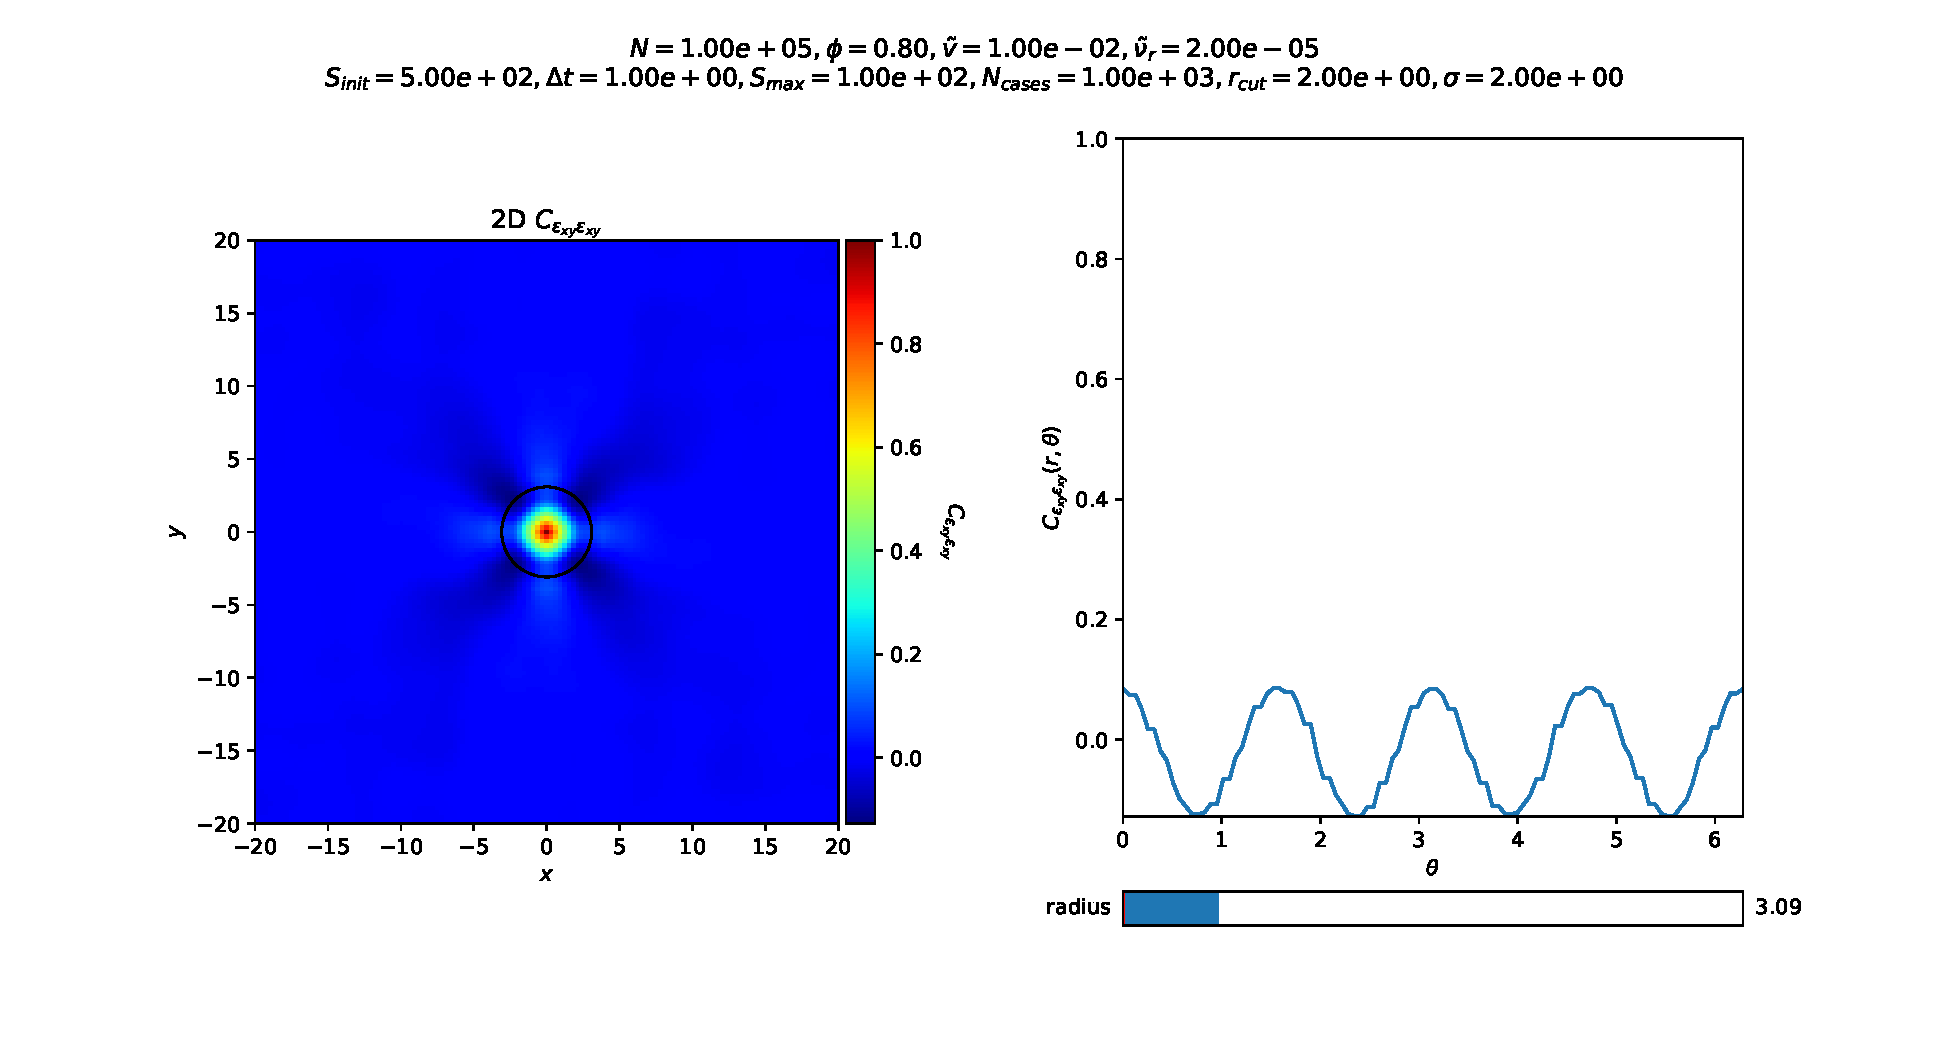
\includegraphics[width=\textwidth]{figures/figs/Cssb_Dk8000_Vj1000_Rg2000_Nq1000_In5000_Tl1000_Ml1000_Co1000_Bn3000_XN1500_Yn1500_grid_circle.eps}
\caption{}
\label{css_map_real_quarter}
\end{figure}

\section{Collective mean square displacement method}

\subsection{Collective mean square displacement}

StackExchange \faStackExchange~ \cite{stackexchange}

\subsection{Results}

\end{document}
